\documentclass[tikz,border=4pt]{standalone}
% Paleta y fuentes compartidas por el libro y las figuras (única fuente de verdad).
\RequirePackage{xcolor}
\definecolor{oxido}{HTML}{B7410E}
\definecolor{cobre}{HTML}{D27D2D}
\definecolor{carbon}{HTML}{2B2B2B}
\definecolor{azul}{HTML}{1F5F8B}
\definecolor{arena}{HTML}{F4EDE4}

\usepackage{fontspec}
\setsansfont{FiraSans}[Extension=.otf,UprightFont=*-Regular,BoldFont=*-SemiBold,ItalicFont=*-Italic,BoldItalicFont=*-SemiBoldItalic]
\setmonofont{FiraMono}[Extension=.otf,UprightFont=*-Regular,BoldFont=*-Medium,Scale=0.95]
\usetikzlibrary{positioning,arrows.meta,calc}
\begin{document}
\sffamily\small
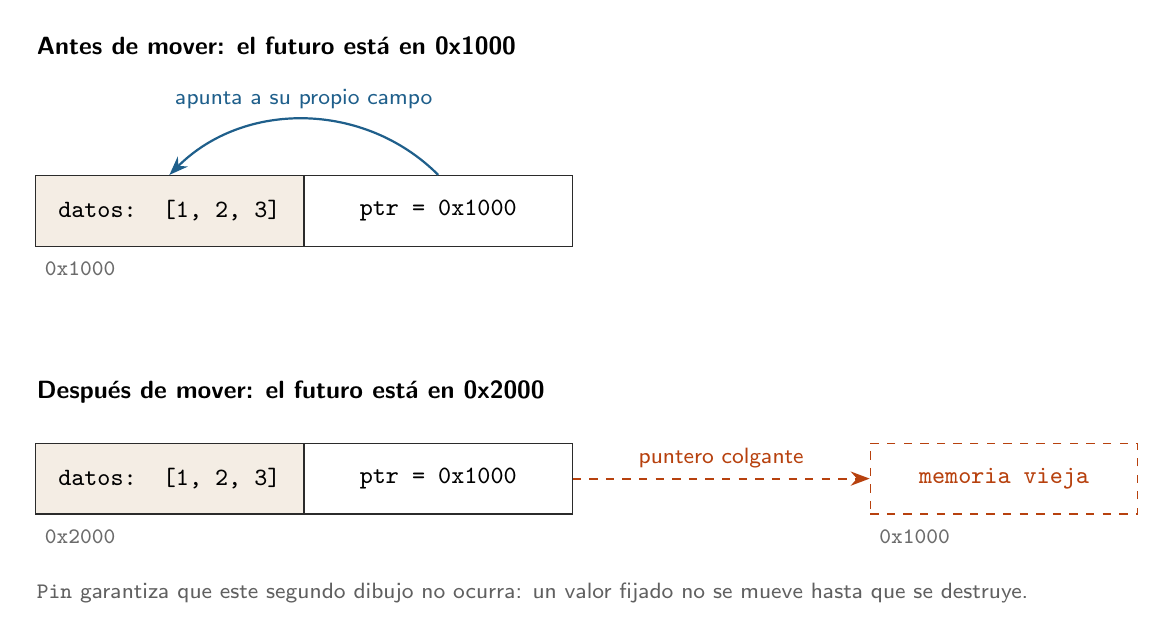
\begin{tikzpicture}[>={Stealth[length=2.4mm]},
  campo/.style={draw=carbon,minimum height=0.9cm,align=center,font=\ttfamily\small},
  dir/.style={font=\ttfamily\footnotesize,text=carbon!70},
  tit/.style={font=\sffamily\bfseries\small,anchor=west},
  nota/.style={font=\sffamily\footnotesize,text=carbon!75,align=left}]
  % Antes de mover
  \node[tit] at (-0.1,2.1) {Antes de mover: el futuro está en 0x1000};
  \node[campo,fill=arena,minimum width=3.4cm,anchor=west] (d1) at (0,0) {datos: [1, 2, 3]};
  \node[campo,fill=white,minimum width=3.4cm,right=0pt of d1] (p1) {ptr = 0x1000};
  \node[dir,below=2pt of d1.south west,anchor=north west] {0x1000};
  \draw[->,thick,azul] (p1.north) to[out=135,in=45] node[nota,above,text=azul] {apunta a su propio campo} (d1.north);
  % Después de mover
  \node[tit] at (-0.1,-2.3) {Después de mover: el futuro está en 0x2000};
  \node[campo,fill=arena,minimum width=3.4cm,anchor=west] (d2) at (0,-3.4) {datos: [1, 2, 3]};
  \node[campo,fill=white,minimum width=3.4cm,right=0pt of d2] (p2) {ptr = 0x1000};
  \node[dir,below=2pt of d2.south west,anchor=north west] {0x2000};
  % Hueco viejo
  \node[campo,draw=oxido,dashed,text=oxido,minimum width=3.4cm,anchor=west] (v) at (10.6,-3.4) {memoria vieja};
  \node[dir,below=2pt of v.south west,anchor=north west] {0x1000};
  \draw[->,thick,oxido,dashed] (p2.east) -- node[nota,above,text=oxido] {puntero colgante} (v.west);
  \node[nota,anchor=north west] at (-0.1,-4.6)
    {\texttt{Pin} garantiza que este segundo dibujo no ocurra: un valor fijado no se mueve hasta que se destruye.};
\end{tikzpicture}
\end{document}
